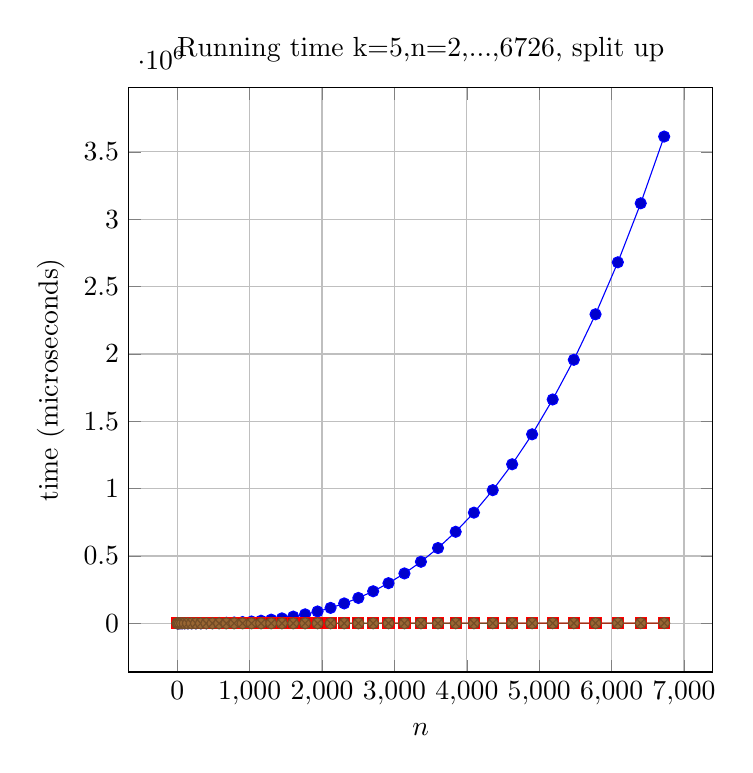
\begin{tikzpicture}
\begin{axis}[
title={Running time k=5,n=2,...,6726, split up},
height=9cm,
width=9cm,
grid=major,
xlabel = $n$,
ylabel = time (microseconds),
]
\addplot coordinates {
%crossing
	(2,0)
	(6,0)
	(18,0)
	(38,1)
	(66,8)
	(102,22)
	(146,45)
	(198,104)
	(258,222)
	(326,447)
	(402,821)
	(486,1444)
	(578,2415)
	(678,3878)
	(786,6006)
	(902,9178)
	(1026,13244)
	(1158,19144)
	(1298,27359)
	(1446,36821)
	(1602,49895)
	(1766,66658)
	(1938,88071)
	(2118,114616)
	(2306,147650)
	(2502,188395)
	(2706,237995)
	(2918,298074)
	(3138,370383)
	(3366,457025)
	(3602,558914)
	(3846,679704)
	(4098,821822)
	(4358,988634)
	(4626,1180886)
	(4902,1403311)
	(5186,1662007)
	(5478,1956547)
	(5778,2294661)
	(6086,2680522)
	(6402,3118674)
	(6726,3614138)
};
\addplot coordinates {
%visibility 
	(2,0)
	(6,0)
	(18,0)
	(38,0)
	(66,0)
	(102,0)
(146,1)
(198,2)
(258,3)
(326,4)
(402,6)
(486,9)
(578,11)
(678,15)
(786,18)
(902,22)
(1026,28)
(1158,33)
(1298,40)
(1446,47)
(1602,56)
(1766,65)
(1938,75)
(2118,87)
(2306,100)
(2502,115)
(2706,131)
(2918,148)
(3138,167)
(3366,190)
(3602,213)
(3846,238)
(4098,264)
(4358,298)
(4626,328)
(4902,363)
(5186,400)
(5478,440)
(5778,481)
(6086,530)
(6402,574)
(6726,628)
};
\addplot coordinates {
%Dijkstra
	(2,0)
(6,0)
(18,0)
(38,0)
(66,1)
(102,2)
(146,4)
(198,6)
(258,10)
(326,15)
(402,21)
(486,28)
(578,36)
(678,46)
(786,59)
(902,71)
(1026,85)
(1158,101)
(1298,121)
(1446,150)
(1602,178)
(1766,207)
(1938,232)
(2118,268)
(2306,305)
(2502,349)
(2706,408)
(2918,453)
(3138,502)
(3366,556)
(3602,620)
(3846,690)
(4098,762)
(4358,830)
(4626,902)
(4902,993)
(5186,1096)
(5478,1182)
(5778,1283)
(6086,1378)
(6402,1496)
(6726,1610)
};
\end{axis}
\end{tikzpicture}
